\chapter{Markov Decision Processes}
\label{chapter2}
\usetikzlibrary{matrix}

\vspace{0.5cm}

\noindent Reinforcement learning refers to both a learning problem and a subfield of machine learning. A typical reinforcement learning setting is depicted in figure~\ref{fig:rlsetting} and, as you can see it, shows a controller and a system continuously connected with each other where the controller receives the state of the system and the reward of the previous iteration and outputs a new action to send to the system. In response to this action, the system makes a transition and this cycle is repeated indefinitely. The main goal of reinforcement learning is to actually learn the problem and manage to control the system in order to maximize the reward. Problems with these characteristics are defined as Markov Decision Processes (MDPs) and the purpose of this chapter is to introduce MDPs as they describe the environment for reinforcement learning.
\begin{figure}[ht]
    \centering
    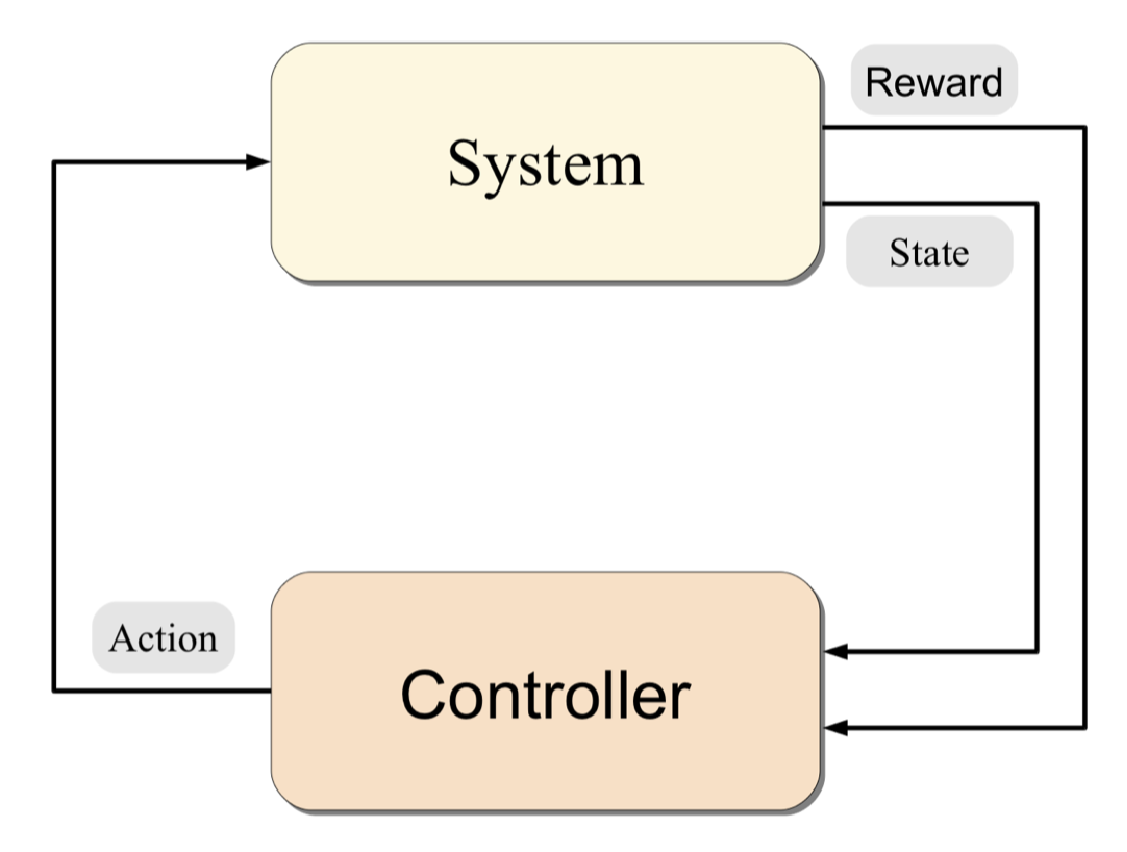
\includegraphics[width=0.6\textwidth]{./pictures/rlsetting.eps}
    \caption{A typical reinforcement learning setting}
    \label{fig:rlsetting}
\end{figure}

\section{Problem Definition}

A Markov Decision Process is defined as a tuple, a triple, a 4-elements tuple or sometimes as a 5-elements tuple, depending on the specifications. In any case, here are the most important elements that define a MDP:
\begin{itemize}
    \item A \textbf{state space} $\mathcal{S}$ which is a countable non-empty set of states $\mathcal{s}$;
    \item An \textbf{action space}  $\mathcal{A}$ which defines a countable non-empty set of actions $\mathnormal{a}$, or $\mathnormal{a(s)}$ if the set of actions is function of the state where we are in;
    \item A \textbf{transition probability distribution} or \textbf{transition model} $\mathcal{P}$ that defines the probability of moving from state $\mathnormal{s}$ to $\mathnormal{s'}$ following action $\mathnormal{a}$. This probability is defined as $\mathbb{P}(s_{t+1} = \mathnormal{s'} \vert s_t = \mathnormal{s}, a_t = \mathnormal{a})$;
    \item An \textbf{immediate reward function} $\mathcal{R}$ which gives the reward received when $\mathnormal{a}$ is chosen in state $\mathnormal{s}$ and can be written as $\mathcal{R}(\mathnormal{s})$ or $\mathcal{R}(\mathnormal{s, a})$ or $\mathcal{R}(\mathnormal{s, a, s'})$;
    \item and a \textbf{discount factor} $\mathcal{\gamma}$ that will be described later.
\end{itemize}

First of all, why are MDPs called Markov Decision Processes? Now that we have the definition, we can explain it. MDPs are a tool for modeling sequential decision-making problems where a decision maker interacts with a system in a sequential way~\cite{RLAlgs}. With this definition, we already explained the \textit{decision} and the \textit{process} part of the name; but why \textit{markovian}?

Well, the \textbf{Markovian property} is a property stating that the conditional probability of the future depends only on the present state and not on past states or, in other words, that the current state where whatever person, computer, system you are trying to model is, is sufficient to decide on future actions and spaces without having to look backwards in time. We can see this in the definition of the transition probability distribution where the conditional probability of $\mathnormal{s_{t+1}}$ is conditioned only by $\mathnormal{s_t}$ and not by $\mathnormal{s_{t-1}}$.

\section{An example}

\begin{figure}[ht]
    \centering
    \includegraphics[width=0.6\textwidth]{./pictures/frozenlake.eps}
    \caption{Frozen Lake. An example of a MDP game~\cite{DeepRLCourse}}
    \label{fig:frozenlake}
\end{figure}

MDPs can be better explained with the game of Frozen Lake depicted in figure~\ref{fig:frozenlake}. The game's story is that a guy was playing frisbee but with a wrong shot his frisbee got stuck in the middle of a frozen lake and it has to be retrieved. The ice is very slippery and so every time a step is made, you have some probability of ending up in a different place. The grid system shows the starting cell, the final cell and some holes where you shouldn't end up.

In this game, the state is the complete grid system with the place where you are marked. There are $4 \times 4$ possible states (all possible cells in the grid) although some of them will be bad states, meaning that if you reach one of those states you "lose". \\
The possible actions are obviously 4, as the possible directions you are able to follow, i.e. LEFT, RIGHT, UP, DOWN. \\
The model instead describes the rules of the game or better, describes what will happen if you do something in a particular place. In this case, since the ice is slippery, when you choose to follow an action you will have $0.5$ probability of going in the correct direction and $0.5$ probability of ending up in a wrong one. \\
For example, given that you are in the top left starting corner, your possible actions are going DOWN or RIGHT. Let us say that you choose DOWN, mathematically you will get formally:
\begin{align*}
    \mathbb{P}(s_{t+1} = DOWN \ \vert \ s_t = START, \ a_t = DOWN) &= 0.5 \\
    \mathbb{P}(s_{t+1} = RIGHT \ \vert \ s_t = START, \ a_t = DOWN) &= 0.5 \\
    \mathbb{P}(s_{t+1} = UP \ \vert \ s_t = START, \ a_t = DOWN) &= 0 \\
    \mathbb{P}(s_{t+1} = LEFT \ \vert \ s_t = START, \ a_t = DOWN) &= 0
\end{align*}
using the notation of $s_{t+1}$ equal to DOWN (RIGHT, UP, LEFT respectively) meaning "the space you would end up into, having moved down (right, up, left respectively) of one cell". \\
We still have to define the reward in the game. Since the goal is a very good cell, the reward of reaching that state would be $+1$ and since all the other cells are just a path to the good cell, they would give reward $0$.

Now that we have seen all the definitions in a game example, the understanding should have become clearer.

\section{The reward function}

We still have to give a closer look to the reward. \\
The reward is a function that maps the space and the action to a real number that can be translated into the \textit{goodness} of your action and can be mathematically written as:
\begin{equation}
    \mathnormal{r(s,a, s')} = \mathbb{E}[\mathcal{R}_{t+1} \ \vert \ S_t = s, A_t = a, S_{t+1} = s']
\end{equation}
since it gives the expected immediate reward.
\newline
\newline
The \textbf{return} is the total discounted sum of the rewards from time step $t$:
\begin{equation}
    \mathcal{R}_{t+1} + \gamma\mathcal{R}_{t+2} + \gamma^{2}\mathcal{R}_{t+3} + \dots = \sum^{\infty}_{k=0}\gamma^k \mathcal{R}_{t+k+1}
\end{equation}
Where the discount $\gamma \in [0,1]$ is the present value of future rewards. Thus, if $\gamma < 1$ then rewards far in the future worth exponentially less than rewards received in the first stages. \\
If $\gamma < 1$ then the MDP is defined as \textit{discounted} MDP instead if $\gamma = 1$ the MDP is \textit{undiscounted}.

We have to explain better the reward function. If $\gamma = 1$ and for every step the reward is positive, then actually the sum from $0$ to $\infty$ is equal to $\infty$. If this is the case, then there is no real gain in changing state since the return at an infinite time step in the future is infinite so it doesn't matter to move now or later. This is the \textit{existential dilemma of immortality} that says: if I have infinite time in the future and I know that moving now or later (making an action) will bring me to infinite reward, why should I move now? \\
This is why the discounted reward is important. It treats rewards nearest to the current time step more with respect to the ones further in the future. The discounted summation has a boundary, in opposition to the undiscounted one: in fact, if we define as $\mathcal{R}_{max}$ the maximum reward for one single step, and hypothetically we say that every step is rewarded with this amount of reward, still the discounted return is bounded by:
\begin{equation}
    \sum^{\infty}_{k=0}\gamma^k \mathcal{R}_{max} = \frac{\mathcal{R}_{max}}{1 - \gamma}
\end{equation}
that is actually a geometrical series and so it can be easily computed. As we can see, if $\gamma$ is close to $0$, the higher boundary is near $\mathcal{R}_{max}$ and when $\gamma$ is near to $1$, the higher boundary becomes bigger and bigger until, for $\gamma = 1$, the result degenerates to $\infty$.

The goal of the system, or decision-maker, is to choose a behavior that maximizes the expected return.

\section{Policy}
The Markov Decision Process as depicted above describes a problem. Given a problem, we always need to find a solution; and a solution for a Markov Decision Process is called a \textbf{policy} $\mathcal{\pi}$. But, \textit{what is a policy?} A policy is a sort of "brain" for the decision maker that tells how to choose actions. There are two kinds of policies:
\begin{itemize}
    \item \textbf{deterministic policies} where the action is just a function of the state:
    \begin{equation}
        a = \pi(s)
    \end{equation}
    \item \textbf{stochastic policies} where the action is a conditional distribution given a state:
    \begin{equation}
        a \sim \pi(a \ \vert \ s)
    \end{equation}
\end{itemize}

An \textbf{optimal policy} is the one the maximizes the long term return.

We'll go more in depth in policies in the next chapter.

\section{Summary}
A Markov Decision process has two main functions, the reward function $\mathcal{R}$ and the transition model function $\mathcal{P}$. This last one suggests the actions to do at each state in order to reach another state while the first one gives rewards after every step to suggest if you are going well or not.

When we have those two functions that is, we can predict which reward will be received and which will be the next state for any state-action pair, the MDP can be solved through Dynamic Programming techniques and the optimal policy can be found. \\
If those two functions can't be computed or are not available, other approaches must be taken and reinforcement learning is the best approach.